\documentclass{article}
\usepackage[utf8]{inputenc}

\usepackage{problems}
\usepackage{graphicx}
\usepackage{todonotes}
\usepackage{enumitem}

\graphicspath{ {./images/} }

\NewTasksEnvironment[label=\Alph*]{tasks2}[\task]

\newcommand{\degree}{\ensuremath{^{\circ}}}
\renewcommand{\angle}{\measuredangle}

\begin{document}

\section{Number Theory}
\subsection{Integer Answer Problems}

\begin{problem}
What is the largest integer that divides $n^3-n$ for all odd $n$?
\end{problem}
\answer{24}

\begin{problem}
How many distinct, real solutions does the equation $\Big((x^2-1)^2-2\Big)^2 = 4$ have?
\end{problem}
\answer{3}

\begin{problem}
How many square numbers are there between $101$ and $10001$?
\end{problem}
\answer{90}

\begin{problem}
What is the sum of all numbers between $1$ and $100$ which are divisible by $3$?
\end{problem}
\answer{1683}

\begin{problem}
At most how many of $12$ consecutive positive integers can be prime?
\end{problem}
\answer{6}

\begin{problem}
How many positive integers are there, that are smaller than three times the sum of their digits?
\end{problem}
\answer{17}

\begin{problem}
Which is the smallest integer $n > 2$ such that $(2^2-1)\cdot(3^2-1) \cdot \ldots \cdot (n^2-1)$ is a square number?
\end{problem}
\answer{8}

\begin{problem}
For a given positive integer $n > 1$, we write down all its positive divisors in ascending order: $1 < d_1 < \ldots < d_k < n$.
How many different $n$ satisfy $d_k = 1111 d_1$?
\end{problem}
\answer{5}

\begin{problem}
Let $n$ be the smallest positive integer, such that $10n$ is a square number and $6n$ is a cube number. What is $n$?
\end{problem}
\answer{36000}


\subsection{Multiple Answer Questions}
\begin{problem}
The expression $n^2+n+41$, for any positive integer $n$, is certainly...
\begin{tasks2}(2)
\task prime
\task bigger than $(n+1)^2$
\task odd
\task not a square
\end{tasks2}
\end{problem}
\answer{C}

\begin{problem}
The number $323$ is...
\begin{tasks2}(2)
\task a prime
\task a square
\task the difference of two primes
\task the difference of two squares
\end{tasks2}
\end{problem}
\answer{D}

\begin{problem}
If $n+9$ is divisible by $6$ but not by $4$, for some integer $n$, it follows that...
\begin{tasks2}(2)
\task $n^2$ is divisible by $9$
\task $n$ is odd
\task $n+5$ is divisible by $6$
\task $n+3$ is divisible by $12$
\end{tasks2}
\end{problem}
\answer{A, B and D}

\begin{problem}
If some positive integers $a,b$ and $c$ satisfy $a^2+b^2 = c^2$, it follows that...
\begin{tasks2}(2)
\task $a+b > c$
\task $c$ is odd
\task $a \neq b$
\task $c$ is not divisible by $7$
\end{tasks2}
\end{problem}
\answer{A and C}

\begin{problem}
\todo{Too hard}
Marco and Tanish each choose an integer $2 \leq x, y \leq 10$ and play the following game: Starting with the number $100$ on the blackboard, if the number is divisible by $x$ they divide it by $x$, otherwise they add $y$. They repeat this process until the number either reaches $1$, and Tanish wins, or it gets greater or equal to $1000$, where Marco wins. If after $1000$ turns neither person has won, the game is declared a draw. Which of the following is true?

\begin{tasks}
\task If Marco picks $3$, he always wins.
\task If Tanish picks $2$, he always wins.
\task
\task
\task 
\task If they pick the same number, Marco always wins.
\end{tasks}
\end{problem}
\answer{f)}

\begin{problem}
There exists a three-digit number $ABC$, such that
\begin{tasks2}
\task{$ABC$ is divisible by $C$ and the two-digit number $AB$}
\task{$ABC$ is divisible by $A$ and the two-digit number $BC$}
\task{$A>C>0$ and $ABC - CBA$ is a prime number} 
\task{$ABC + BCA + CAB = 2021$}
\end{tasks2}
\end{problem}
\answer{A}

\newpage

\section{Geometry}
\subsection{Integer Answer Questions}

\begin{problem}
What is the sum of all the interior angles of a hexagon?
\end{problem}
\answer{720}

\begin{problem}
Let $\alpha$ be the smallest angle in some triangle. What is the maximal value $\alpha$ can take?
\end{problem}
\answer{60\degree}

\begin{problem}
If the diagonal of square $A$ is $16$ times as large as the perimeter of square $B$, how many times as large is its area?
\end{problem}
\answer{32}

\begin{problem}
A circle is inscribed inside an equilateral triangle, which in turn is inscribed in another circle. If the area of the small circle is $17$, what is the area of the big one?
\end{problem}
\answer{68}

\begin{problem}
If a right angled triangle has a side of length $15$ and a side of length $12$, what is its smallest possible area?
\end{problem}
\answer{54}

\begin{problem}
Let $P$ be a point inside the rectangle $ABCD$. If $|AP| = 6$, $|BP| = 2$ and $|CP| = 7$, how long is $|DP|$?
\end{problem}
\answer{9}

\begin{problem}
Let $P$ be a point inside the equilateral triangle $ABC$ of height $100$. If the distances from $P$ to the lines $AB$ and $BC$ are $23$ and $35$ respectively, how far is $P$ from the line $CA$?
\end{problem}
\answer{42}

\begin{problem}
Quirin has $3$ sticks of length $12$. He breaks exactly one of them into two sticks and arranges all five sticks to a right-angled triangle. How big is the area of that triangle?
\end{problem}
\answer{96}

\begin{problem}
Tanish folds a rectangular piece of paper twice. He then cuts it with a scissor along a straight line. How many pieces of paper can he produce at most ?
\end{problem}
\answer{5}


\subsection{Multiple Choice Questions}
\begin{problem}
Given is a square $ABCD$ in the plane. How many squares are there that share exactly two vertices with $ABCD$?
\end{problem}
\begin{tasks}(5)
\task 4
\task 6
\task 8
\task 12
\task 16
\end{tasks}
\answer{d)}

\begin{problem}
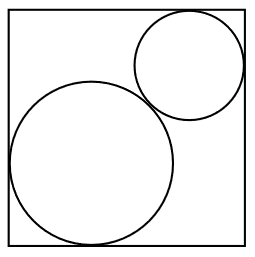
\includegraphics[width=70pt]{img3} \\
Two circles are inscribed in a square of sidelength $1$, as shown in the picture above. What is the sum of the two radii?
\end{problem}
\begin{tasks}(2)
\task $\dfrac{1}{2}$
\task $\dfrac{1}{\sqrt{2}}$
\task $\sqrt{2} - 1$
\task $2 - \sqrt{2}$
\task The value depends on the radii.
\end{tasks}
\answer{d)}

\begin{problem}
$ABCD$ is a square of side length $1$. The circles of radius $1$ with centers $B$ and $C$ intersect in $P$ and the circles of radius $1$ with centers $A$ and $D$ intersect in $Q$. What is the length of the segment $|PQ|$?
\end{problem}
\begin{tasks}(5)
\task $2- \sqrt{2}$
\task $\dfrac{3}{4}$
\task $\sqrt{5} - \sqrt{2}$
\task $\dfrac{1}{\sqrt{3}}$
\task $\sqrt{3} - 1$
\end{tasks}
\answer{e)}

\begin{problem}
For each triangle, we compute the circumference $c$ and the sum of the three altitudes $d$ and set $M=c \cdot d$. Which of the following statements are true?
\end{problem}
\begin{tasks2}
\task For every triangle it holds that $c > d$.
\task There exists a triangle of area $1$ such that $M$ is bigger than $100$
\task There exists a triangle of area $1$ such that $M=18$.
\task For every triangle of area $1$, $M>6$ is satisfied
\end{tasks2}
\answer{A,B,C,D}

\subsection{Multiple Answer Questions}

\begin{problem}
Which statements about the following configuration must certainly hold?\\
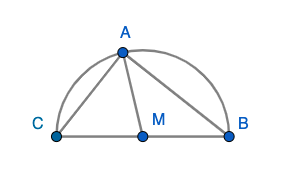
\includegraphics[width=200pt]{img1}
\begin{tasks2}(2)
\task $\angle CAM = \angle ABC$
\task $\angle AMC = 2\angle ABC$
\task $\angle ACB + \angle ABC = 90\degree$
\task $Area(ACM) = Area(AMB)$
\end{tasks2}
\end{problem}
\answer{B, C and D}

\begin{problem}
Which statements about the following configuration must certainly hold?\\
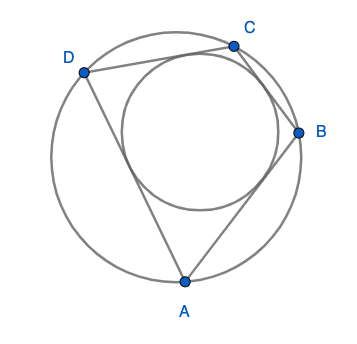
\includegraphics[width=200pt]{img2}
\begin{tasks}(2)
\task $|AC| = |BD|$
\task $|AB|+|CD| = |BC|+|DA|$
\task $\angle ABC +\angle ADC = 180\degree$
\task $|AB|+|BC| = |AD|+|DC|$
\task $\angle CBD = \angle ACB$
\task $\angle ABD = \angle ACD$
\end{tasks}
\end{problem}
\answer{b), c) and f)}

\begin{problem}
How many distinct intersections could arise from drawing $5$ different, infinitely long, straight lines?
\begin{tasks2}(4)
\task $3$
\task $4$
\task $5$
\task $6$
\end{tasks2}
\end{problem}
\answer{B, C and D}

\newpage

\section{Combinatorics}
\subsection{Integer Answer Questions}

\begin{problem}
In how many ways can $8$ people form $4$ teams of $2$ people each?
\end{problem}
\answer{105}

\begin{problem}
In a finite sequence consisting of the letters A,B,C and D, any two distinct letters can be found next to each other at least once. What is the minimal length of the sequence?
\end{problem}
\answer{8}

\begin{problem}
How many three-digit numbers are there such that no odd digit is to the left of an even digit?
\end{problem}
\answer{425}

\begin{problem}
On an infinite chessboard, there is a chess piece. In a move, the piece goes to an adjacent square in any of the four directions. On how many different squares can it end up after $6$ moves?
\end{problem}
\answer{49}

\begin{problem}
Quirin writes a non-negative integer in each square of a $3 \times 3$ table, such that the six sums of the rows and columns are all different. What is the smallest possible value that the sum of all numbers can attain?
\end{problem}
\begin{tasks}(5)
\task 6
\task 7
\task 8
\task 9
\task 10
\end{tasks}
\answer{c)}

\begin{problem}
How many ways are there to go from one vertex of a cube to the opposite corner, travelling along the edges, without passing through a vertex twice?
\end{problem}
\answer{18}

\begin{problem}
How many ways are there to go from one vertex of a cube to the opposite corner using 3 edges?
\end{problem}
\answer{6}

\begin{problem}
On a table there are nine pebbles of weights $10$, $20$, $\ldots$, $90$. How many possibilities are there to choose four pebbles that can be partitioned into two groups of equal weight?
\end{problem}
\answer{41}

\begin{problem}
How many ways are there for a chess piece to move from the bottom left to the upper right corner on a $5\times 5$ chess board, assuming the piece can only move to the right and upwards in a straight line?
\end{problem}
\answer{70}

\begin{problem}
In how many different ways can a $2\times 11$ rectangle be filled with $11$ indistinguishable dominoes of size $1\times 2$?
\end{problem}
\answer{144}

\subsection{Multiple Choice Questions}

\begin{problem}
How many ways are there to number the edges of a cube with numbers from 0 to 11 so that the sum of the edges at each vertex is odd? 
Note: two configurations are considered equal if you can turn the cube to make them identical. If reflection is necessary, they are considered different. 
\end{problem}
\begin{tasks}(2)
\task 0 
\task $(6!5!)\cdot 4$
\task $(6!5!)\cdot 6$
\task $(6!5!)\cdot 12$
\task $(6!5!)\cdot 24$
\task $12!$
\end{tasks}
\todo{I don't like this kind of question. Should be smaller numbers and integer answer}
\answer{I think it's b...?}

\subsection{Multiple Answer Questions}
\begin{problem}
Let $O$ be the number of possible ways to number the edges of a cube with numbers from 0 to 11 so that the sum of the edges at each vertex is odd, and $E$ similarly defined so that the sums at all vertices is even. Which of the following statements are true?
Note: two configurations are considered equal if you can turn the cube to make them identical. If reflection is necessary, they are considered different. 
\end{problem}
\begin{tasks}(3)
\task $O > E$
\task $\frac{O}{E} \in \mathbb{N}$
\task $O < E$
\task $\frac{E}{O} \in \mathbb{N}$
\task $O = E$
\task $O \cdot E = 0$
\end{tasks}
\answer{b), d) and e).}

\begin{problem}
Herr Euler has a class of 26 children, all of whom are boys or girls. Which of the following must be true?
\end{problem}
\begin{tasks}(1)
\task There are two girls born in the same month.
\task There are two boys born in the same month.
\task There are two children of the same gender born in the same month.
\task There are two children of different gender born in the same month.
\task There are three children born in the same month.
\task In some five consecutive months, fewer than 11 children are born.
\end{tasks}
\answer{c), e) and f).}

\begin{problem}
In the country of Abecid, every child is given a name with an even number of letters where vowels and consonants alternate, but the letter Y was removed from the alphabet in 1837 after the Great Vowel-Consonant Dispute. Which of the following is true?

\todo{Idk what to put here but I really wanna use the fact that $2\cdot20^n\cdot5^n$ is a really round number.}
\begin{tasks}(2)
\task 
\end{tasks}
\answer{}
\end{problem}
 
\begin{problem}
There are $51$ distinct positive integers on the blackboard, none exceeding $100$. Which statements about this board must be true?
\begin{tasks2}
\task There are two consecutive numbers
\task There are two numbers differing by $50$
\task There are two numbers summing to $100$
\task There are six numbers with the same last digit
\end{tasks2}
\end{problem}
\answer{A, B and D}

\begin{problem}
\todo{Too hard}
Arnaud has a loaded die, where the probabilities of each face coming up are not necessarily equal. He is going to roll the die twice and Tanish is going to bet on the difference between the two numbers. Which of the following could be the most probable?
\end{problem}
%\todo{This problem is clearly too hard (if you want to be sure your answer is correct) for the first round but the solution is too inelegant to be a proof-based question. But maybe we can find another way to formulate it that is not too hard, so I leave it here for the others to think about. In any case through simple logic (all values equal) you could guess that b) is correct, if one face is certain to come up then a) is clearly correct, and finding the construction for c) is not too hard (all even faces have one-third chance, for example). Being sure that d, e, f don't work requires AM-GM or simpler algebra ideas however, but seeing that d never works could be intuitive...?}
\begin{tasks}(6)
\task 0
\task 1
\task 2
\task 3
\task 4
\task 5
\end{tasks}
\answer{a), b) and c).}

\begin{problem}
\todo{too hard}
Tanish and Raphael are playing a game which works as follows: Firstly, they start at the number 42. Then they take alternating turns, performing the following operations on the number: 
\begin{itemize}
    \item On Tanish's turn, he may add 2 to the number, or he may pass.
    \item On Raphael's turn, he may divide the number by 2 if it is even, or add 3 if it is odd, or he may pass.  
\end{itemize}
Tanish wins if the number is exactly equal to 1 or greater than 100, and Raphael wins if the number is exactly equal to 99.  However, if they both pass on consecutive turns, the second person to pass loses. They both play perfectly.
Which of the following is true?
\begin{tasks}
\task If Tanish starts, he can guarantee victory.
\task If Raphael starts, he can guarantee victory.
\task Raphael cannot win at the end of his own turn. 
\task You can always avoid losing if you start.
\task If you are not starting, you always lose.
\task The game is always drawn. 
\end{tasks}
\answer{ c), d), f)}
\end{problem}

\begin{problem}
You have a large collection of cows, which are either male or female and Swiss or foreign. You know the probability of a cow in your collection being male, and the probability of female cow in your collection being Swiss. After counting all your cows, which of the following could you deduce?
\todo{reformulate with ratios instead of probabilities}
\begin{tasks}
\task The number of male Swiss cows.
\task The number of female Swiss cows.
\task The number of foreign cows.
\task The probability that a Swiss cow is male
\task The probability that male cow is Swiss.
\task The probability that a cow that is not foreign \textbf{and} female happens to be male.
\end{tasks}
\end{problem}
\answer{b), f)}

\section{Miscellaneous}
\subsection{Integer Answer Questions}

\begin{problem}
The average of ten different positive integer is $10$. What is the maximal possible value of the largest of these numbers?
\end{problem}
\answer{55}

\begin{problem}
What does the expression
$$1000\cdot\left(\frac{1}{1\cdot 2} + \frac{1}{2\cdot 3} + \cdots + \frac{1}{99\cdot 100}\right)$$
evaluate to?
\end{problem}
\answer{990}

\begin{problem}
What does the expression
$$1000\cdot\left(1-\frac{1}{2^2}\right)\cdot\left(1-\frac{1}{3^2}\right)\cdots\left(1-\frac{1}{100^2}\right)$$
evaluate to?
\end{problem}
\answer{505}

\subsection{Multiple Choice Questions}

\begin{problem} %yeah, it's super easy, but we need super easy problems :) 
The sum of five consecutive integers equals the sum of the three next bigger numbers. What is the biggest of these eight numbers?
\end{problem}
\begin{tasks}(5)
\task 4
\task 8
\task 9
\task 11
\task 12
\end{tasks}
\answer{d)}

\begin{problem}
You have two analogue 12-hour clocks, one of which gains a minute each day and one of which loses a minute each day. If they agree right now, how many days later will they show the same time again?
\end{problem}
\begin{tasks}(2)
\task 60
\task 360
\task 720
\task 1440
\task 3600

\end{tasks}
\answer{b)}


\subsection{Multiple Answer Questions}

\begin{problem}
Let $A,B,C$ and $D$ be different statements. We know that if $A$ is false, $B$ must be true. Additionally, if $B$ and $C$ both are true, then so is $D$. What can we definitely conclude?
\begin{tasks2}(2)
\task All statements could be true
\task All statements could be false
\task If $B$ is false, then $A$ is true
\task $A$ and $D$ can both be true
\end{tasks2}
\end{problem}
\answer{A , C and D}

\begin{problem}
The five friends $A$, $B$, $C$, $D$ and $E$ are playing a social deduction game. Good guys always have to tell the truth and bad guys always have to lie. This is their conversation:
\begin{enumerate}[label=\Alph*:]
    \item "C and D are either both good or both bad." 
    \item "If E is good, A is telling the truth!"
    \item "There is an even number of bad guys in the game."
    \item "At least one among A, B and C has to be bad."
    \item "A and C are not both good."
\end{enumerate}
Which of the following statements are true?
\end{problem}
\begin{tasks2}
\task It is possible that $A$ and $C$ are both good
\task $D$ is certainly good
\task $B$ is certainly bad
\task It's possible that there is only one good player
\end{tasks2}
\answer{A, B, C}

\newpage
\section{Additional easy questions (all topics)}

\begin{problem}
What is the greatest value achievable using all the numbers $1,2,3,4,5$ and all the operations $+,-,\times,\div$ exactly once each as well as parentheses?
\end{problem}
\answer{35}

\begin{problem}
Tim forgot the last five letters of his password. He only knows that they are some combination of the capital letters $A, B$ and $C$. How many possibilities does he have to take into consideration?
\end{problem}
\answer{243}

\begin{problem}
What is the smallest integer greater than $1$ which is both a square and a cube?
\end{problem}
\answer{64}

\begin{problem}
What integer has the property that if you square it and subtract $49$ you get the same thing as if you first subtract $49$ and then square it?
\end{problem}
\answer{25}

\begin{problem}
Cyril has $6$ different candy bars. In how many possible orders can he eat them all?
\end{problem}
\answer{720}

\begin{problem}
Jana has four cards with the numbers $2$, $5$, $7$ and $9$ written on them. She orders them in a row. Then she computes the product of the numbers on the first two cards, subtracts the number on the  third card and multiplies the result by the number on the last card. What is the biggest possible result she can obtain in the end?
\end{problem}
\answer{305}

\begin{problem}
Tanish thinks of an integer $1\leq n \leq 100$ and Marco wants to guess the number. After each guess, Tanish tells him whether his guess was correct, too small or too big. What is the smallest number of guesses that can guarantee Marco to win, assuming he guesses smartly?
\begin{tasks} (5)
\task 4
\task 5
\task 6
\task 7
\task 8
\end{tasks}
\end{problem}
\answer{d)}

\begin{problem}
Viviane writes down a four digit number. She notices that if she takes away the second digit, she gets a three digit number which is exactly $\dfrac{1}{9}$ of the original number. Which of these numbers could she have written down at the beginning?
\begin{tasks} (5)
\task 2365
\task 8811
\task 7291
\task 3690
\task 1575
\end{tasks}
\end{problem}
\answer{e)}

\begin{problem}
Four real numbers $a,b,c$ and $d$ satisfy the equation $a^2b^2 + c^2d^2 + a^2c^2 = 0$. One of the following equations is not necessarily true. Which one?
\begin{tasks}(3)
\task $abc + bcd = 0$
\task $ab + cd = 0$
\task $abcd = 0$
\task $ac + bd = 0$
\task $abd + acd = 0$
\end{tasks}
\end{problem}
\answer{d)}

\begin{problem}
Arnaud and Valentin are playing a game. Starting with $n$ stones on the table, they alternatingly remove either $1$ or $2$ stones with Arnaud starting. The player who removes the last stone wins. For which $n$ can Valentin definitely win?
\begin{tasks2}(4)
\task 4
\task 6
\task 11
\task 24
\end{tasks2}
\end{problem}
\answer{B and D}

\begin{problem}
All the numbers from $1$ up to $10$ are written on the blackboard. David now repeatedly replaces two numbers by their (positive) difference until only one number is left. What could this number possibly be?
\begin{tasks2}(4)
\task 0
\task 1
\task 6
\task 11
\end{tasks2}
\answer{B}
\end{problem}

\begin{problem}
There are $100$ coins in a line, all showing heads. Louis now turns every, then every second, then every third and so on up to every $100$th coin. Assuming that the first coin was flipped every time, how many coins show heads at the end?
\end{problem}
\answer{91} %isn't it 90?

\begin{problem}
Paul made less than $200$ cookies and now wishes to distribute them into paper bags, such that each bag has exactly the same number of cookies. Sadly, this never seems to work out: If he wants to distribute them into $5$ bags, there are four cookies left. The same thing happens if he wants to distribute them into $6$ bags. If he wants to have $7$ bags, there are $3$ cookies left. How many cookies did Paul make in total?
\end{problem}
\answer{94}

\begin{problem}
Henning's favourite ice cream store offers $8$ different flavours. This time, Henning wants to order three scoops of ice cream but he wants to have at least two different flavours. How many possibilities does he have to do this?
\end{problem}
\answer{112}

\begin{problem}
Julia and Florian independently think of an integer between $1$ and $10$. Julia says: "No matter what number you chose: If we compute the product of our two numbers, it will not contain the digit $6$.". Florian says: "Alright, then the sum of our numbers must be $14$." What is Florian's number?
\end{problem}
\begin{tasks}(5)
\task 4
\task 5
\task 6
\task 8 
\task 9
\end{tasks}
\answer{e)}

\begin{problem}
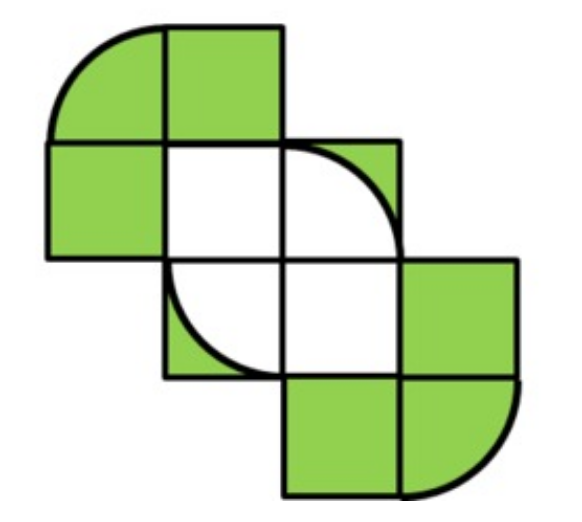
\includegraphics[width=150pt]{img5} \\
Using her compass, Rada drew this figure on a grid paper. If the side length of one small square is $2$, what is the green area?
\end{problem}
\begin{tasks}(5)
\task $12$
\task $16$
\task $16 + 2\pi$
\task $24$
\task $24 + 2\pi$
\end{tasks}
\answer{d)}

\begin{problem}
Raphi von Winti draws three circles on the empty blackboard. What is the maximal number of connected regions created?
\end{problem}
\answer{8}

\begin{problem}
On Monday, I bought a lot of chocolate bars. On Tuesday, I ate two of them and gave exactly half of the remaining ones to my friend. On Wednesday, I ate exactly a third of the remaining chocolate bars and gave three to my sister. On Thursday, I ate the three remaining chocolate bars. How many did I buy on Monday?
\end{problem}
\answer{20}

\begin{problem}
How many integers are there between $10$ and $1000$ that stay the same when the order of their digits is reversed.
\end{problem}
\answer{99}

\begin{problem}
There are $16$ dots arranged in a regular $4\times 4$ grid. How many possible squares can you draw by connecting $4$ dots using straight lines?
\end{problem}
\answer{20}

\begin{problem}
What is the total area of the following figure composed of $4$ congruent, right triangles? \\
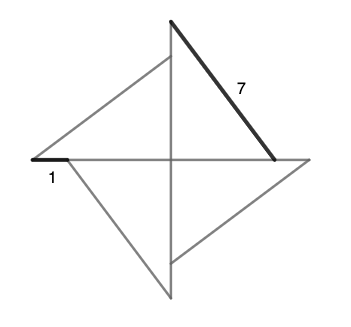
\includegraphics[width = 5cm]{img6.png}
\end{problem}
\answer{48}

\begin{problem}
If every internal angle of a polygon is greater than $123\degree$, what is its minimal number of vertices?
\end{problem}
\answer{7}

\begin{problem}
Valentin is raising pigs and geese on his farm. One day, he counts the total number of legs as being 100 (not including himself). He then goes to the market and sells some pigs and then uses some of the money he just made to buy geese. He comes back and adds them to the farm; to his surprise, there are still 100 legs on his farm. If a pig sells for 5 dollars and you can buy a goose for 2 dollars, and he made 10 dollars, how many pigs did he sell?
\end{problem}
\answer{10}

\begin{problem}
Anaëlle plays a little mathematics game with his little brother. It starts with the number $1$ on the blackboard. In each step, her brother can choose to multiply the number on the board by $2,3$ or $5$ and replace the number by the result of this mulitplication. How many numbers are possible after the fourth step?  
\end{problem}
\begin{tasks}
\task 15
\task 18
\task 21
\task 24
\task 27
\end{tasks}
\answer{a)}

\begin{problem}
On a cube, we label each of its faces and vertices with $1$ and each edge with $-1$. What is the total sum of the labels?
\end{problem}
\begin{tasks}
\task 0
\task 2
\task 4
\task 6
\task 8
\end{tasks}

\begin{problem}
What is the remainder of $2^2 \times 3^3 \times 5^5 \times 7^7$ when divided by $8$?
\end{problem}
\begin{tasks}
\task 2
\task 3
\task 4
\task 5
\task 7
\end{tasks}

\begin{problem}
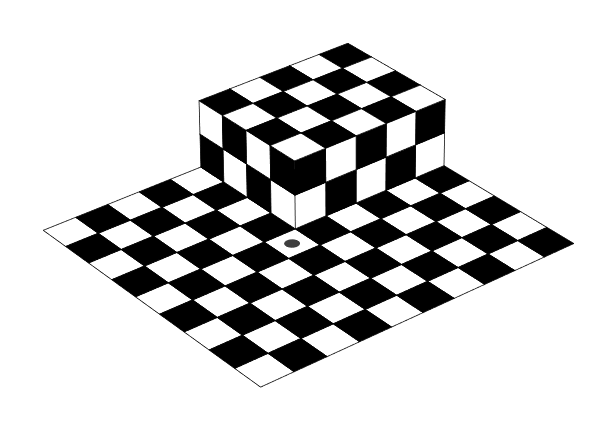
\includegraphics[width=250pt]{2021/First Round/images/img7.png}
An ant is initially on the square marked with the black dot. The ant moves across an edge from one square to an adjacent square four times and then stops. How many of the possible finishing squares are black?
\end{problem}

\begin{problem}
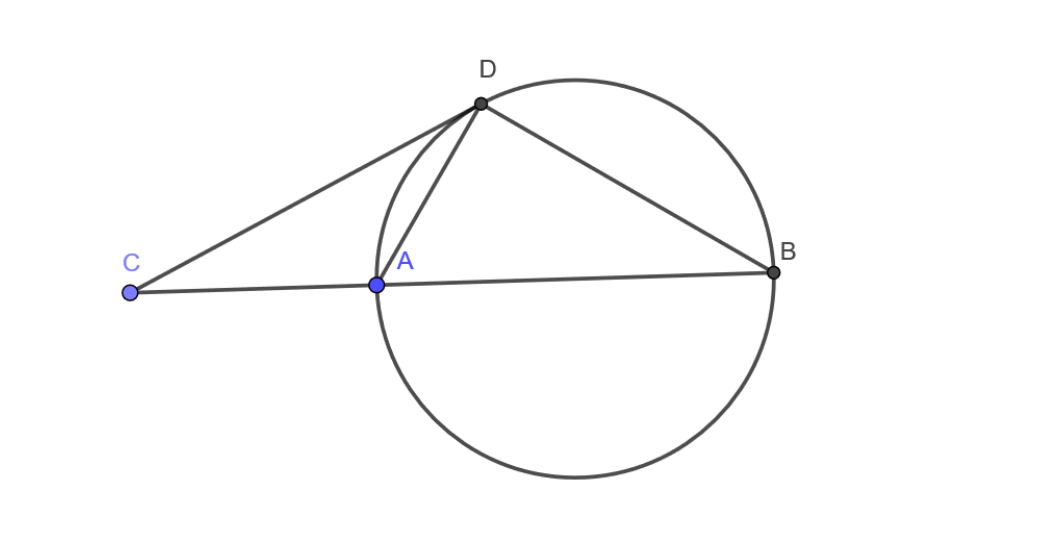
\includegraphics[width=250pt]{2021/First Round/images/img8.png}
$AB$ is the diameter of a circle, $C$ is on the line $AB$ and $CD$ is a tangent to the circle. If $|CA|=68$, $|AD|=48$ and $|DB|=90$, what is the length of $CD$?
\end{problem}




\end{document}


